%!TEX root=../../../template.tex
\subsection{Collection System}%
\label{sub:methods_collection}

The flight controller unit is in permanent communication with the
collection system, through the spectrometer controlling computer. This
is an \gls{rpi}-based single board device. This equipment controls the
spectral acquisition process, which is conducted by an Avantes Mini
spectrometer with 2048 channels and a \gls{usb} 3.0 connection. The
Avantes spectrometer can be interfaced with both Unix-based and
Microsoft Windows operating systems through a set of software libraries
that are available for download at this manufacturer's website. There
are several physical interfaces for available for both types of
operating system. Nowadays, the most common and expedient way to run
this connection is through the \gls{usb} port. This is also the
connection that allows a higher data throughput (allowing smaller
integration times to be used). In the end, the proposed system will only
run in Unix-based computers, but the Windows version was very important
for initial experiments, which at the time were programmed in C\# (code
included in Appendix~\ref{ap:c_sharp_spectrometer}). The spectrometer
control flow is very different in the two approaches. The Unix version
works by continuously polling the spectrometer for the spectral data,
which is the somewhat obvious strategy. The Windows version uses a
sophisticated technique: Windows messages. This is a set of fixed-value
event flags that are fired at the Operating System level and can be
intercepted by running programs.

This type of spectrometer is usually shipped with an \gls{SMA}
connector, for direct connection of a fibre optics cable. While this is
ideal as a bench-top solution and when size and weight restrictions are
looser, we found it not to be the best fit for our particular case. We
tend to think of fibre optics as an almost lossless medium for data
transmission. This is, of course, true, but it does not hold for its
connectors. They represent one of the most significant sources for
signal loss in an optics fibre line. Avantes does not mention any value
for \gls{SMA} connector losses, but the traditional figure that appears
in most manufacturer's catalogues is around 1dB~\cite{diamond2021,
Optics, amphenol2002}. To test how a direct connection fares when
compared to a fibre connection, I designed a spectrometer support that
can be attached to the telescope via its red-dot rail and fabricated it
using a 3D printer. Technical drawings available in
Appendix~\ref{ap:technical_drawing_telescope_spectrometer_coupling}.

The assembly is displayed in Figure~\ref{fig:direct_vs_optical_assmbly}.
In this experiment, I have found differences of around xx\%\todo{check
this value} between the fibre optics cable and a direct measurement in
which the light goes directly from the telescope into the spectrometer's
connector. These results are plotted in
Figure~\ref{fig:direct_vs_optical_plot}.

\begin{figure}[htpb]
    \centering
    \begin{subfigure}{.45\textwidth}
        \includegraphics[width=\textwidth]{img/pdf/fibre.png}
        \caption{This assembly uses a traditional fibre optics
        connection to transport light between the telescope and the
        spectrometer.}
        \label{fig:fo_light}
    \end{subfigure}
    \hfill
    \begin{subfigure}{.45\textwidth}
        \includegraphics[width=\textwidth]{img/pdf/direct.png}
        \caption{This assembly allows light to pass directly from the
        telescope to the spectrometer.}
        \label{fig:direct_light}
    \end{subfigure}
    \caption{Conducted experiment to evaluate advantages of using a
    direct light connection instead of fibre optics. The spectrometer
    support (that can be seen in red) was designed in Autodesk Inventor and
    3D printed.}%
    \label{fig:direct_vs_optical_assmbly}
\end{figure}

\begin{figure}[htpb]
    \centering
    \missingfigure{}
    \caption{Plots obtained through the collection of light managed by
    the assemblies depicted in
    Figure~\ref{fig:direct_vs_optical_assmbly}}.%
    \label{fig:direct_vs_optical_plot}
\end{figure}

Circumventing the optical loss of signal is normally feasible just by
selecting a more powerful light source. In our case, this would equate
to the selection of a larger telescope, which would go against our size
and weight constraints. Therefore, we had to solve the problem through a
direct light connector that coupled the telescope to the spectrometer's
entrance. This design was made with Autodesk's Inventor CAD software
suite~\footnote{Thanks to a very generous protocol between Autodesk and
many universities around the world that makes this software free for all
FCT NOVA's students.} and some renderings of the designs can be seen in
Figure~\ref{fig:spectrometer_telescope_coupling_3d}. Technical drawings
are also available in
Appendix~\ref{ap:technical_drawing_telescope_spectrometer_coupling}.

\begin{figure}[htpb]
    \centering
    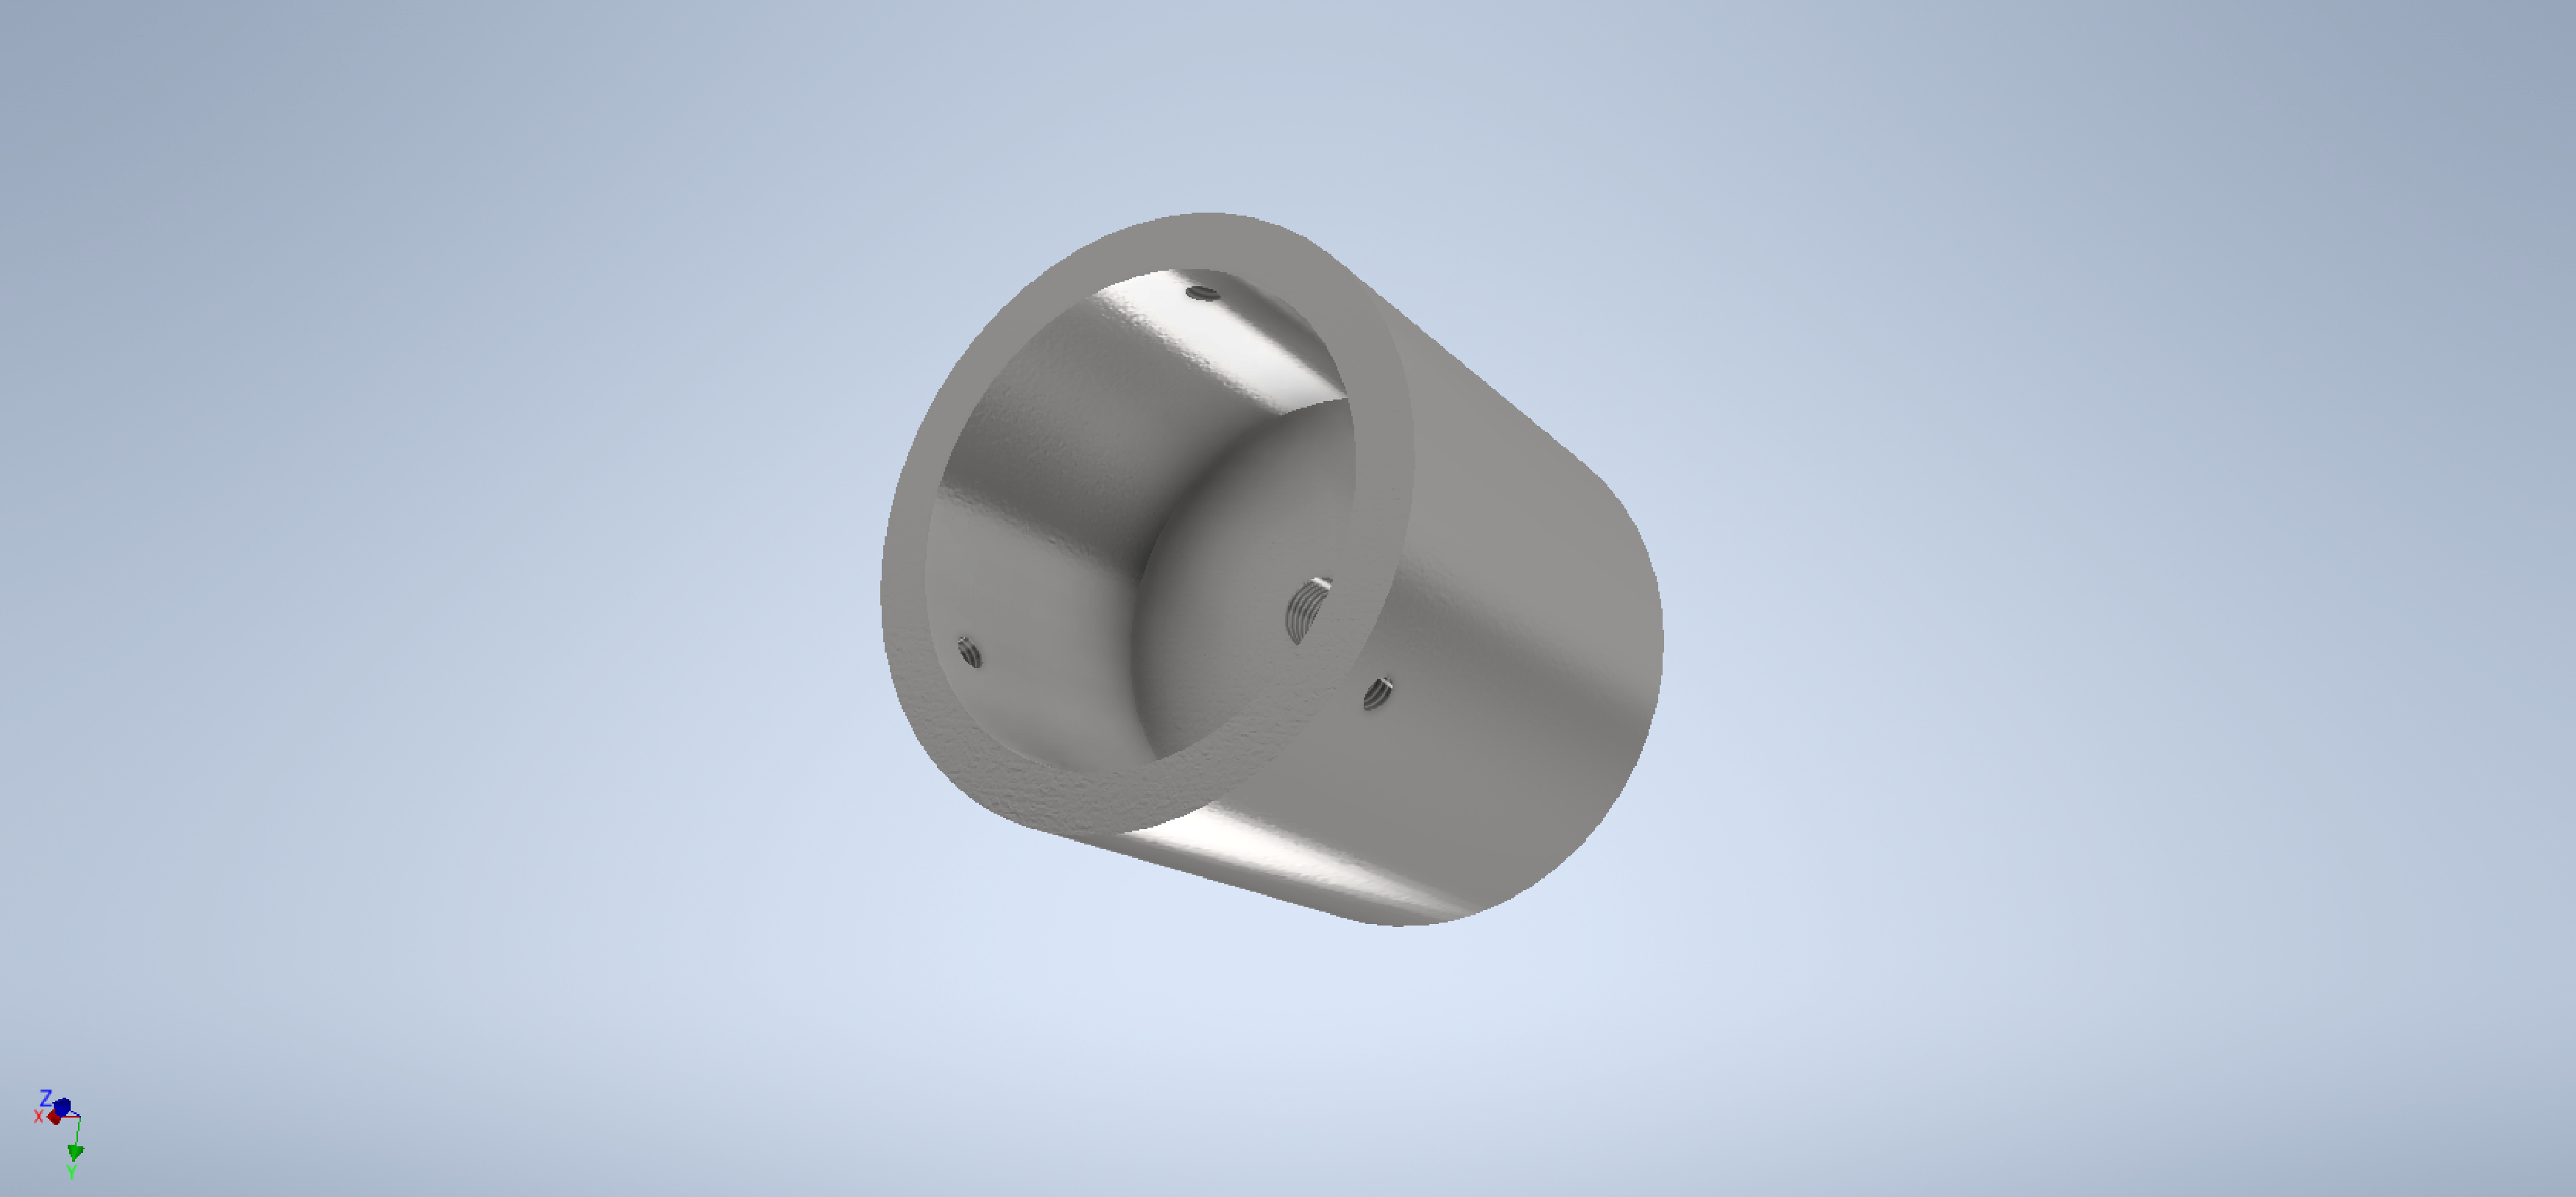
\includegraphics[width=\textwidth]{img/pdf/eyepieceAdapter.pdf}
    \caption{Telescope - Spectrometer coupling. 3D design rendered
    through Autodesk Inventor.}%
    \label{fig:spectrometer_telescope_coupling_3d}
\end{figure}

The centrepiece of this collection system is of course the telescope.
From the beginning of the project, I understood that this was going to
be one of the most important aspects of the endeavour. It has gone
through some iterations before reaching the final design solution. The
telescopes with which I began my experiments were some of the ones used
in the \gls{FFF} project, which were normally Meade ET90 or similar
(90mm diameter Maksutov-Cassegrain telescopes). These seemed too bulky
to mount on a drone. They would fit, of course, but movement would
become a very probable problem. Looking for alternatives at the time
rendered no results. The 90mm diameter telescope market has a lot of
competition, but smaller tubed reflecting telescopes are somewhat rare.
On the refractors side of things, the problem was otherwise. Telescopes
are usually built to look at the skies. Manufacturers try to offer the
best balance between magnification, image quality and ease of use in
each price range. Therefore, commercial refractor telescopes were too
long to include in our drones, as they reached for larger focus lengths
to get more magnification power. Our needs were in fact quite
different. We wanted the light collection capabilities of a telescope
tube, but since our idea was to connect it to a spectrometer, optical
quality was not at all a priority, and neither was magnification. With
this in mind, I started working on a custom made tube design.

I started by choosing the appropriate tube diameter. On a cloudy but
luminous day, I used an ET90 to capture the spectrum that I show in
Figure~\ref{fig:cloudy_but_luminous_day}. This spectrum was collected
with the Avantes Mini spectrometer, with an integration time of 50 ms.
The Poissonian nature of light entering a telescope allows me to assume
that its relationship with time is linear. Moreover, we know that the
quantity of light that enters the telescope varies with the square of
its diameter. Thus we can write the calculations in
Equation~\ref{eq:light_capture}.

\begin{figure}[htpb]
    \centering
    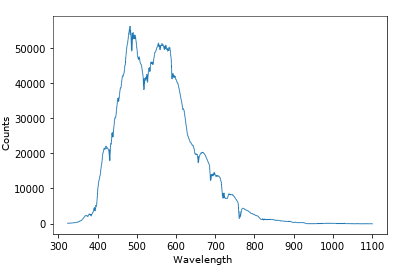
\includegraphics[width=\textwidth]{img/png/ex_spectrum.png}
    \caption{The spectrum captured on a cloudy but luminous day using
    the ET90 telescope and the Avantes Mini spectrometer.}%
    \label{fig:cloudy_but_luminous_day}
\end{figure}

\begin{equation}
    \label{eq:light_capture}
    E \propto D^2 \Leftrightarrow \frac{E_{90}}{E_{25}} =
    \frac{90^2}{25^2} \approx 13
\end{equation}

The same spectrum of Figure~\ref{fig:cloudy_but_luminous_day} would take
13 times longer to collect with a telescope that had 25mm instead of
90mm diameter. In other words, 650 ms. This is a reasonable compromise
given our application.

The first design attempt was a Maksutov-Cassegrain telescope. However,
this was quickly abandoned due to 1) calculations indicated an
impossible length for this kind of telescope and a 25mm diameter; and 2)
the inherent complexity of these telescopes made assembling one
prohibitively costly in terms of time.

The second design was much simpler. It was a refracting tube with the
same diameter (25mm) and a focal length of 300mm. Designs for this
telescope and its optical simulation were produced using OSLO-EDU
software and are included in Appendix~\ref{ap:telescope_design}. This
ended up not being the telescope used in the final design, because as I
was working in this part of the project, Omegon released their MightyMak
60, a 60mm diameter Maksutov-Cassegrain telescope that is small enough
to be fitted onto a drone assembly. This was a perfect timing because
the commercial availability of a suitable telescope allowed significant
time savings on the whole ordering, assembling and testing process. The
specifications of the new telescope are included in
Table~\ref{tab:omegon}~\cite{Omegon2021}.

% Please add the following required packages to your document preamble:
% \usepackage{booktabs}
\begin{table}[]
\centering
\caption{Specifications table for the Omegon MightyMak 60 telescope~\cite{Omegon2021}.}
\label{tab:omegon}
\begin{tabular}{@{}lll@{}}
\toprule
\textbf{Feature}                      & \textbf{Value} & \textbf{Unit} \\ \midrule
\textbf{Aperture}                     & 60             & mm            \\
\textbf{Focal Length}                 & 700            & mm            \\
\textbf{f/}                           & 11,7           & N/A           \\
\textbf{Maximum Useful Magnification} & 120            & x             \\
\textbf{Weight}                       & 0,6            & kg            \\ \bottomrule
\end{tabular}
\end{table}
